\section{Roofline Model}


Our method for evaluating core architecture usage is a simplified variant of the roofline model \cite{williams2009}. 
We start with two key boundaries: 
On the one hand, the maximum memory bandwidth of the system across various arithmetic intensities (AI) creates the diagonal ``roofline''. 
While temporary performance spikes might occur with optimal cache usage, this diagonal represents our realistic bandwidth limit. 
On the other hand, the chip's peak computational performance establishes a firm upper boundary, represented by the horizontal line (Figure~\ref{figure:core-architecture}).

Once we measure our code's throughput and performance, we can draw lines parallel to these two thresholds matching our observations. 
The implementation is considered efficient as long as it performs within $C_{\text{bw}} \geq 80\%$ or reasonably efficient as long as it remains within $C_{\text{bw}} \geq 60\%$ of these maximum values.

Visually, our thresholds create 60\% and 80\% corridors beneath the maximum thresholds. 
The ideal zone is where these corridors intersect (Figure~\ref{figure:core-architecture}). 
A performance within the corridor under the peak if fine, too.
However, we will rarely find such a code in practice.
Being close to the peak bandwidth is might also fine, as we might have an intrinsically memory-bound algorithm.



\paragraph{Data collection}

\begin{figure}[htb]
 \begin{center}
  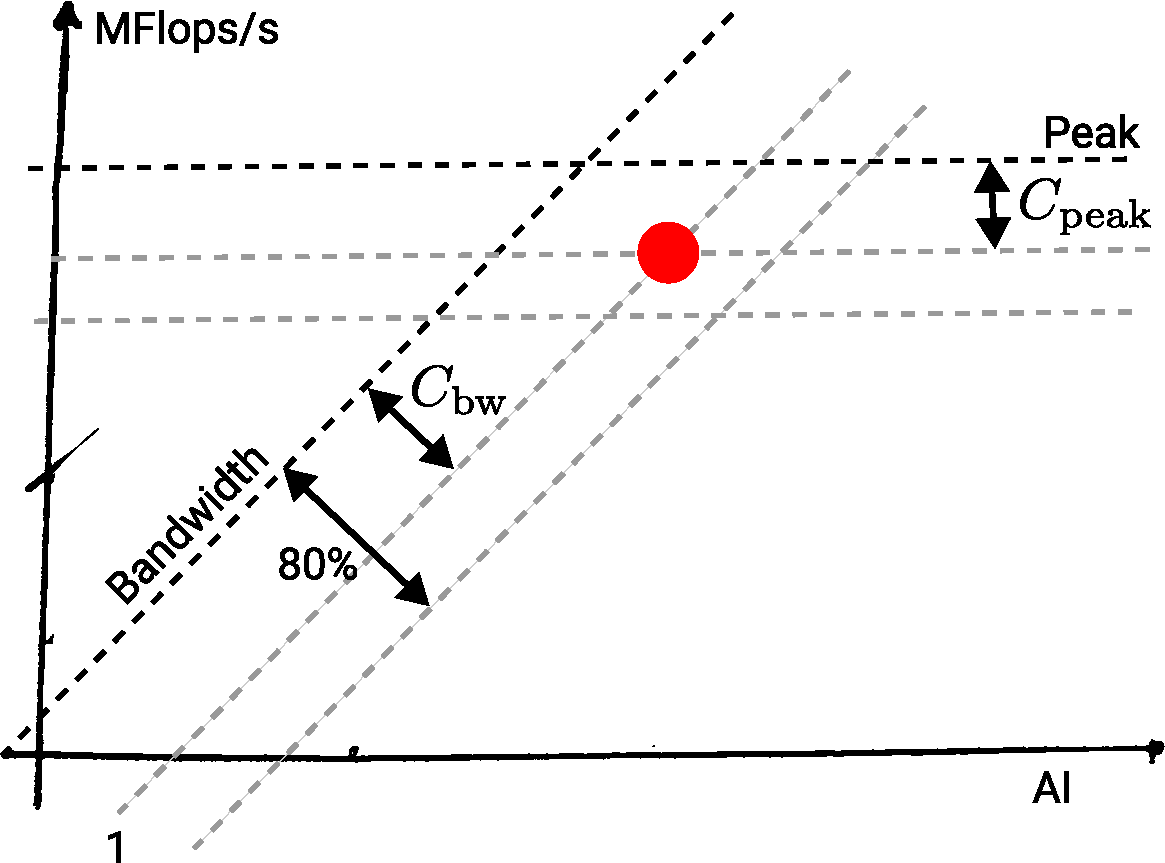
\includegraphics[width=0.7\textwidth]{high-level/core-architecture.pdf}
 \end{center}
 \caption{
  Schematic illustration of a roofline analysis of a code.
  We illustrate the peak performance threshold (dark dotted horizontal line) and the maximum bandwidth (diagonal).
  The code's actual compute performance delivered and memory bandwidth used is by a factor of $C_{\text{peak}}$ or $C_{\text{bw}}$ respectively lower than these maximum thresholds.
  \label{figure:core-architecture}
 }
\end{figure}

Realistic bounds for the roofline are easy to obtain through a number of tools.
The ``only'' tricky bit is how we calibrate the memory bandwidth.
Memory interconnects are designed to serve all hardware threads on their chips.
We will not be able to assess if we use them efficiently if we use only one
core, as we will simply not be able to saturate the theoretical bandwidth with
only of of these.
Therefore, we typically run the benchmark over the whole node
and then divide the throughput by the number of cores to obtain a realistic threshold for a single core.
